This section aims to explore the hardware setup and constraints, outlining key components and requirements for the system and toolsets, and concluding with a summary of the architectures and designs to aid in the subsequent implementation and testing phases.

\subsection{System Equipment \& Design Constraints}
\label{designconstraints}

The system follows from the hardware constraints and assumptions that were set by Shepherd. In this prototype system, as Figure \ref{fig:submersible} illustrates, a plywood plate fastens the custom-fabricated and watertight tubes. The larger of the two tubes houses the Optoma ML550 projector, which features an LED lamp enabling a brightness capability of up to \SI{500}{\lumen}, illuminating a \SI{1}{\centi\metre} DLP for a native resolution of 1280x800, with a maximum \SI{120}{\hertz} vertical and \SI{100}{\kilo\hertz} horizontal scan rate capabilities. The smaller tube houses the RPi 5 (\SI{8}{\giga\byte} RAM variant) SBC, using a Broadcom BCM2712 \SI{2.4}{\giga\hertz} quad-core 64-bit Arm Cortex-A76 CPU to feature an advertised 2-3x performance upgrade from the RPi 4 that Shepherd used.

Connected to this RPi, via a 4-lane Mobile Industry Processor Interface (MIPI) transceiver, is an RPi global shutter (GS) camera, featuring the Sony IMX296LQR-C 1.58MP sensor. Instead of a GS sensor, Shepherd employed the RPi High-Quality (HQ) sensor, however, due to the reasons which Section \ref{designrec} outlines, the GS sensor replaces this. The GS camera uses a PT361060M3MP12 lens, with an adjustable F1.2 aperture, a \SI{6}{\milli\metre} adjustable focal length for a minimum object distance of \SI{0.2}{\metre}, and a field of view of \SI{63}{\degree}. Mounting all components within their respective tubes with 3D-printed mounts, such that the separation between the camera and projector lenses is \SI{12}{\centi\metre}. At the backside of each tube is a metallic cap with watertight cable couplers to pass through the RPi and projector power cables, and an ethernet cable for the RPi.

\begin{figure}[H]
    \centering
    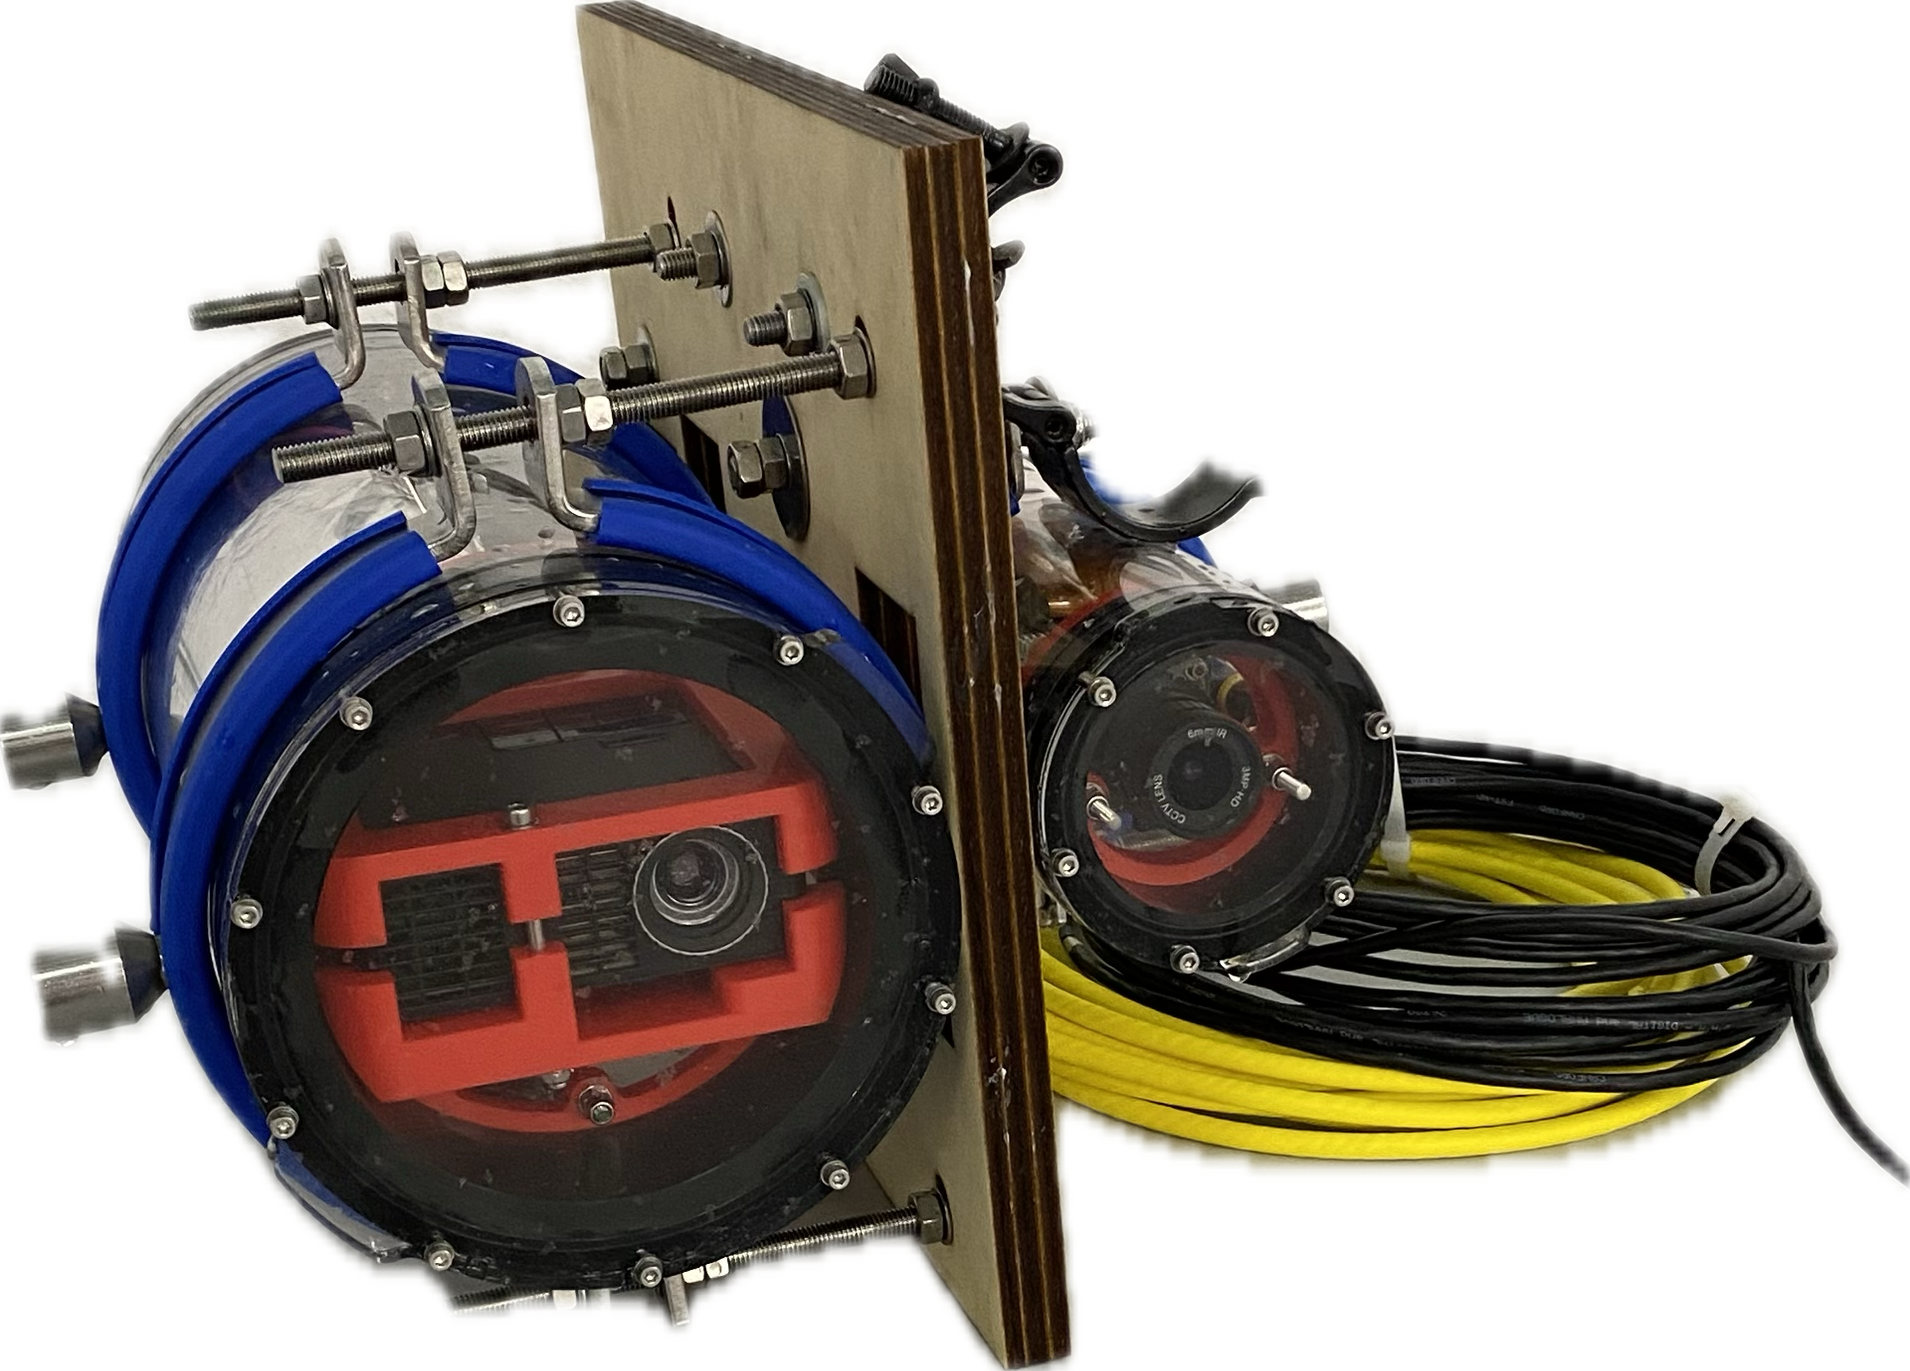
\includegraphics[width=0.8\textwidth]{assets/submersible.png}
    \caption{The submersible system.}
    \label{fig:submersible}
\end{figure}

The design relies on two assumptions: (a) the system is to run below the ocean twilight zone, which is approximately \SI{200}{\metre} below the surface, ensuring the scene is only lit by the system and not other sources such as sunlight, and (b) there are no internal reflections from the housing, such as from the plastic tubes and tube lenses, ensuring all noticeable reflection to be backscatter particles. Due to its watertight construction, disassembling and reassembling the housing is a laborious process, often requiring the reapplication and testing of seals, which can extend the downtime to multiple days. Therefore, this project must prefer conducting tests using pre-recorded footage or synthetic simulations of backscatter to minimise disruptions and maintain operational efficiency.

\subsection{Simulating Backscatter for Synthetic Ground Truth}
\label{designsim}

Given the substantial weight of the submersible, manoeuvring the system into position within an underwater testing tank presents significant challenges during testing. Moreover, the availability of the underwater testing tank at the Institute for Safe Autonomy wasn't fully realised until the later stages of this project. Consequently, there is a need for software capable of synthetically generating a simulation of backscatter particles. Since this simulation is entirely software-based, it must produce ground truth data comprising a dataset, assigning each backscatter particle with a unique ID, allowing for the tracking of coordinates across every frame of the simulation. Comparing the detected backscatter positions from the system with the true positions derived from the simulation ground truth enables the accurate assessment of the system's accuracy and performance.

Employing a straightforward model involving bubbles rising from the bottom of the screen can form a sufficient simulation of random backscatter particle movement in all axis directions: horizontal (x), vertical (y), and towards the camera (z). The simulation can depict backscatter particles as a white circle against a black background for simplicity, with user control over these exact colours. The model should also take into account the bubble expansion due to the pressure difference as they ascend from underwater. As a result, a separate model to simulate bubble distance from the camera location may not be necessary. It's also crucial to model horizontal bubble movement to capture the full range of particle motion.

\subsection{Recording Lossless Video for Physical Testing}
\label{designrec}

At the start of this project, Ben provided me with a GoPro recording from a submersible capturing the seabed, intending to use it as test material to develop the system. However, due to the GoPro's heavy video compression, coupled with its rolling shutter sensor, the video contains a large number of compression artefacts and significant motion blur, as Figure \ref{fig:gopro} illustrates. These issues significantly complicate the task of identifying individual backscatter particles for segmentation, with the system in Figure \ref{fig:submersible} originally, in Shepherd's work, employing an RPi HQ sensor, which is also a rolling-shutter sensor. The limitations posed by the GoPro footage proved the necessity for a GS sensor, prompting the exploration and subsequent implementation of the RPi GS camera. In order to capture test footage using this system, there must be a program in place to record the `raw' footage from the camera, directly from the sensor inside the submersible without any lossy compression.

\begin{figure}[H]
    \centering
    \begin{subfigure}{.49\textwidth}
        \centering
        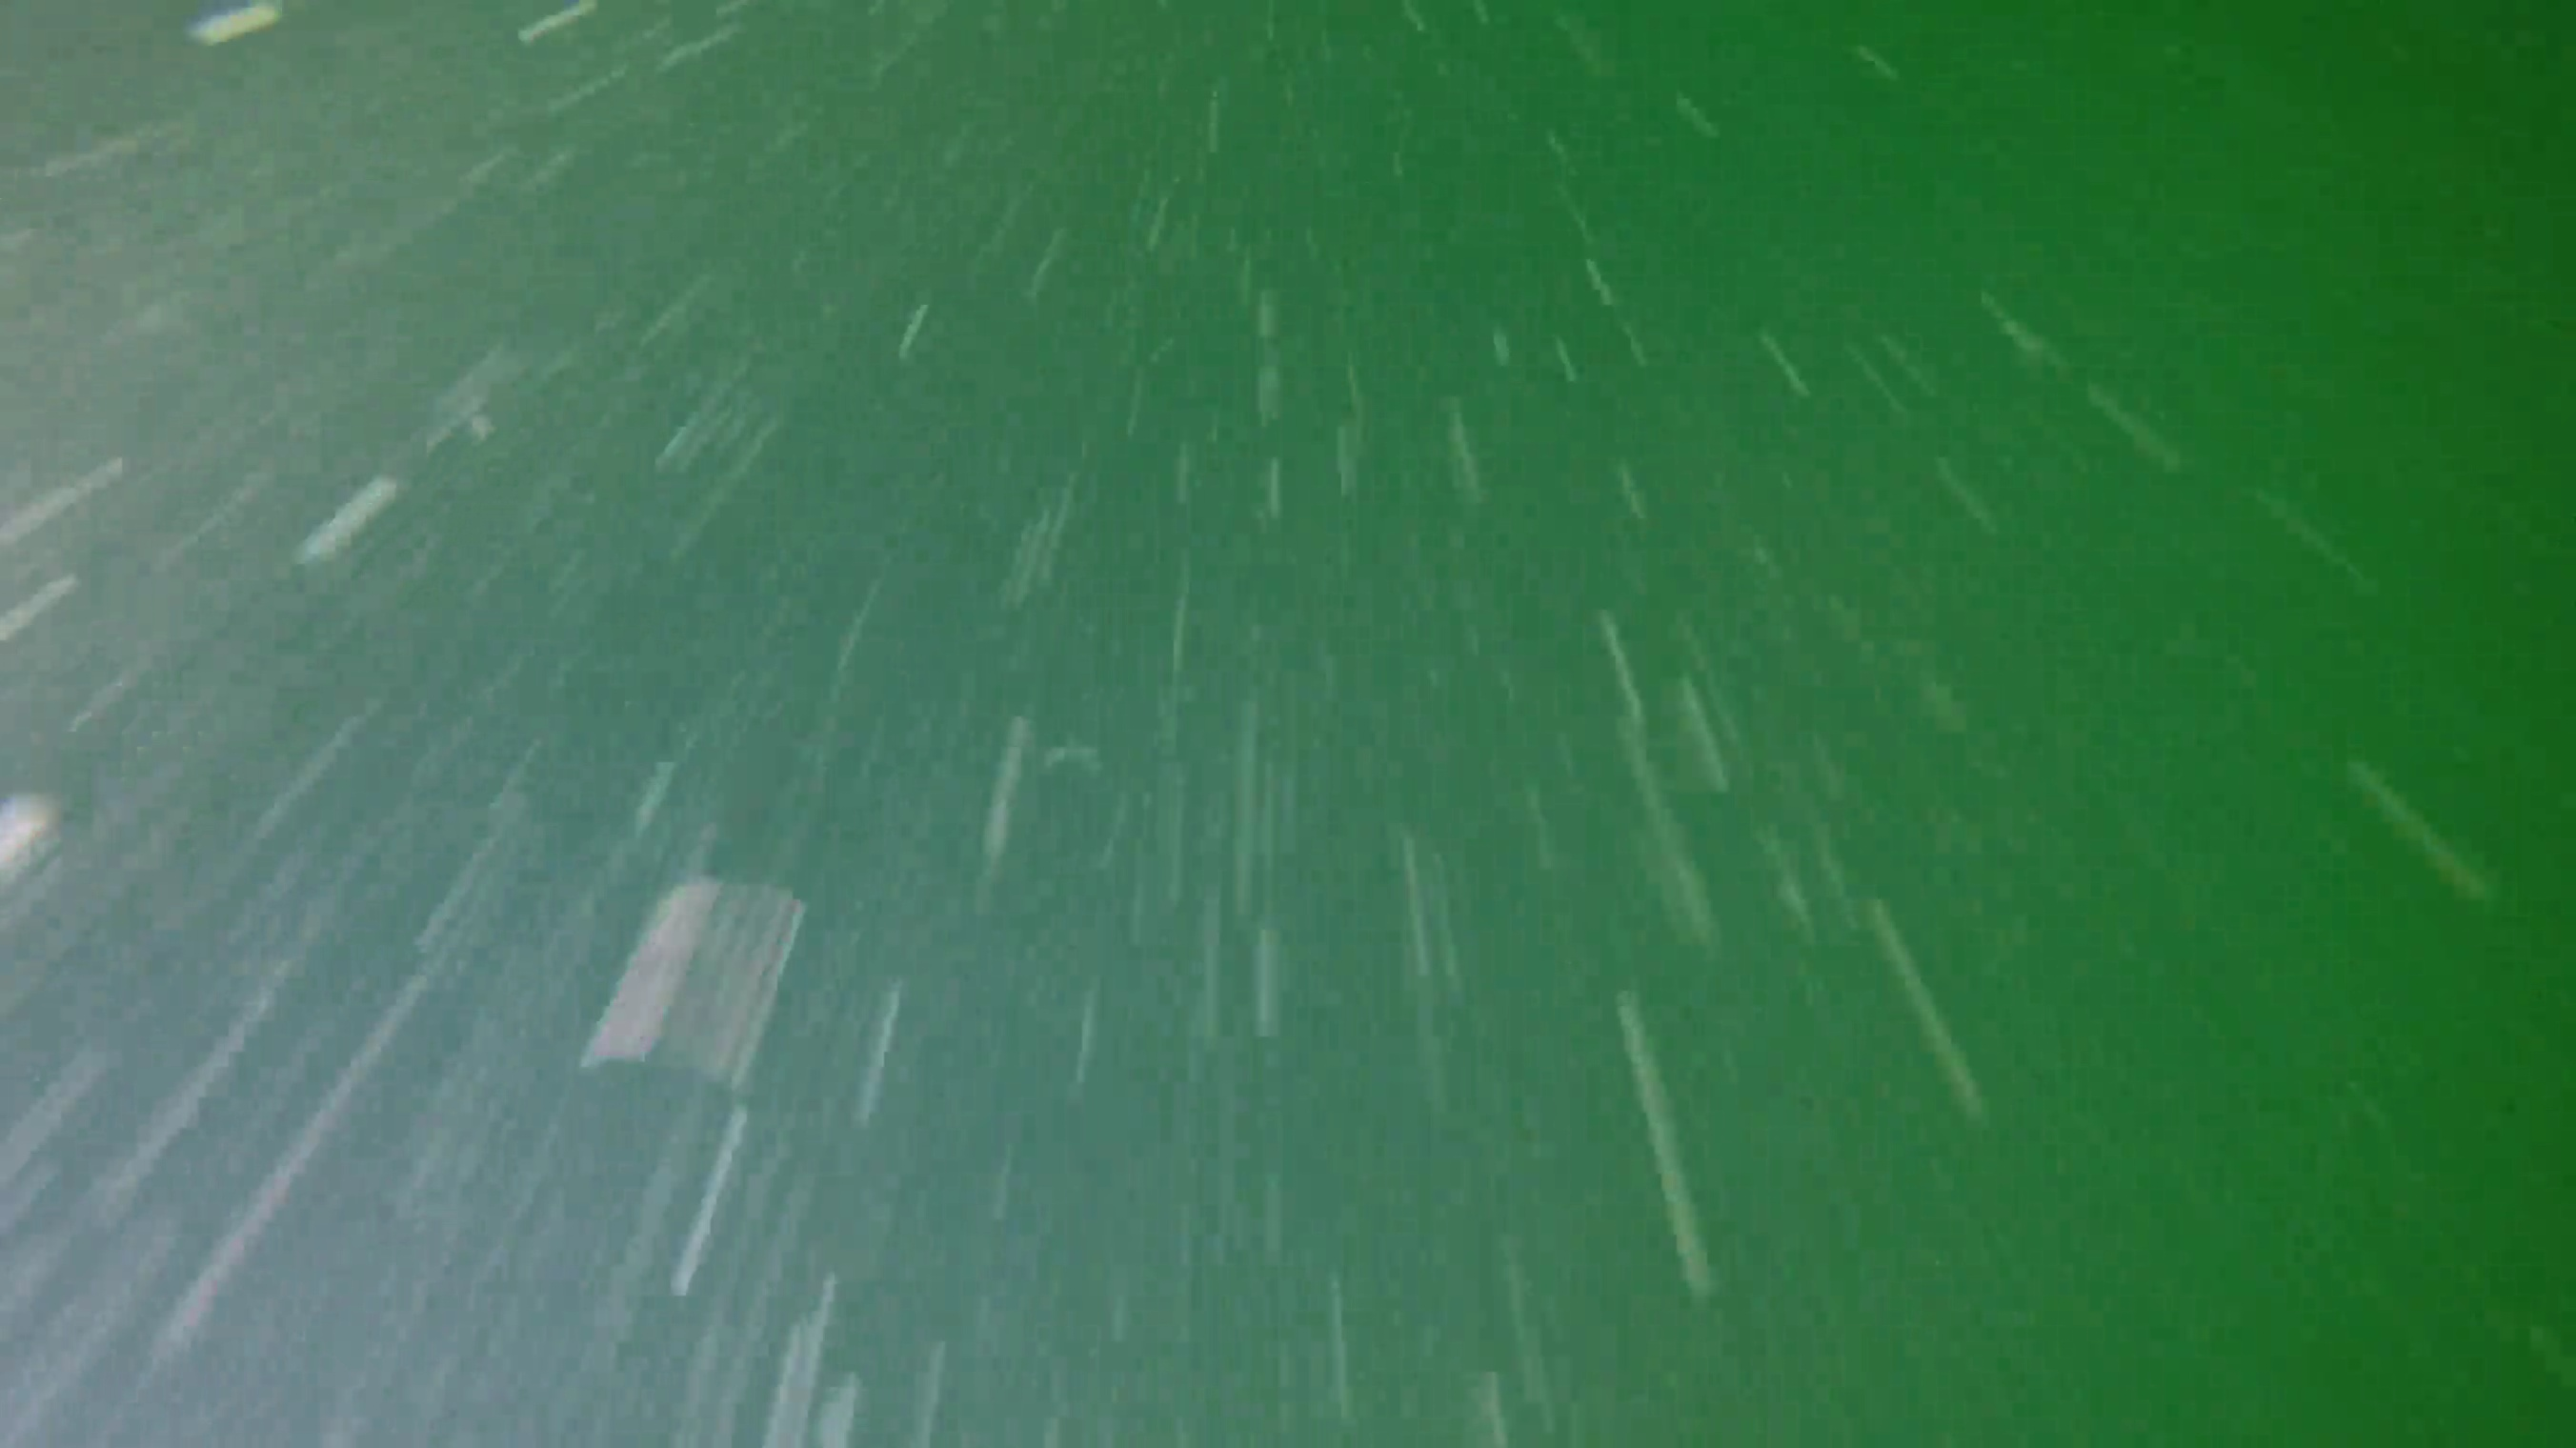
\includegraphics[width=1\linewidth]{assets/gopro_footage_streaks.jpg}
        \caption{}
        \label{fig:motionblur}
    \end{subfigure}
    % \hfill
    \hfill
    \begin{subfigure}{.49\textwidth}
        \centering
        
\includegraphics[width=1\linewidth]{assets/gopro_footage_artefacts.png}
        \caption{}
        \label{fig:artefacts}
    \end{subfigure}
    \caption{Frames from the GoPro footage: (\ref{sub@fig:motionblur}) showing the motion blur of backscatter particles, and (\ref{sub@fig:artefacts}) showing the pixelation artefacts (depending on your display, you may have to look closely to see the pixelation effect).}
    \label{fig:gopro}
\end{figure}

When recording in raw format, the RPi GS camera captures in full 1456x1088 sensor resolution at the maximum compatible framerate of 60 frames per second, using the native RAW10 SBGGR10 Bayer format, which utilises four channels, one red, one blue, and two green, with a 10-bit depth for each. Equation \ref{eq:raw_data_per_frame} calculates the total number of bytes per frame and Equation \ref{eq:raw_data_per_second} calculates the total number of bytes per second when recording in this raw format, where $R_w$ and $R_h$ are the resolution width and height, $D_b$ is the bit depth per channel, $N_{ch}$ is the number of channels, $F_b$ is the number of bits and $F_B$ the number of bytes per frame, $F_{rate}$ is the frame rate, and finally, $S_b$ is the number of bits and $S_B$ the number of bytes per second.

\begin{align}
    \begin{split} \label{eq:raw_data_per_frame}
        F_b & = (R_w \times R_h \times D_b \times N_{ch}) \\
        & = (1456 \times 1088 \times 10 \times 4) \\
        F_b & = \SI{63365120}{\bit} = \SI{63.36512}{\mega\bit} \\
        F_B & = \SI{7920640}{\byte} = \SI{7.92064}{\mega\byte} 
    \end{split} \\
    \notag \\
    \begin{split} \label{eq:raw_data_per_second}
        S_b & = (F_b \times F_{rate}) \\
        & = (63365120 \times 60) \\
        S_b & = \SI{3801907200}{\bit} = \SI{3.8019072}{\giga\bit} \\
        S_B & = \SI{475238400}{\byte} = \SI{475.2384}{\mega\byte} 
    \end{split}
\end{align}

The calculations reveal an approximate transfer rate of \SI{475}{\mega\byte} per second when recording the raw footage, presenting a significant data throughput requirement. It would be impossible to transfer at that data rate to the boot drive due to CPU bottlenecks, and most importantly, boot drive write-speed bottlenecks, with the drive being a USB 3.1 stick. To address this challenge, it is imperative to implement a memory buffer in RAM to temporarily store the recording data, offloading data to the boot drive only once the recording concludes ensuring the system solely reserves the CPU for recording. Additionally, employing functionality to modify resolution for downscaling and to adjust the framerate, effectively further reducing the output filesize without introducing video artefacts.

\subsection{Underwater Backscatter Cancellation System}
\label{designsystem}

The system must employ an image processing pipeline, Figure \ref{fig:processing_pipeline} illustrates this pipeline from a high-level perspective. The pipeline must begin with a greyscale filtering stage to reduce image dimensionality by categorising pixels by brightness, ensuring a single-channel output, reducing processing complexity for the subsequent pipeline stages. The next stage applies a Gaussian blur to reduce noise and small-scale variations in pixel intensities, to improve the edge detection performance such that the edge detection algorithm only detects regions of interest. Post-noise-smoothening, a histogram equalisation stage can improve the dynamic range, enhancing image contrast by redistributing pixel intensities to fully utilise the intensity range. The histogram equalisation stage can drastically improve the edge detection algorithm due to the improved contrast between objects of interest. Application of the Canny algorithm will extract all edges, ideally of the backscatter in isolation due to the previous stages, aiding in the next stage, which is backscatter segmentation. The segmentation stage will utilise a simple methodology, such as highlighting closed-loop edges, in order to isolate and pinpoint the backscatter particles.

Given Python's high-level abstraction, there is a theoretical limit to how close to real-time the system can operate. For this system, I will be targetting a total processing duration, which is the time it takes to capture the frame, apply the image processing pipeline, and finally segment the backscatter particles, of \SI{33.33}{\milli\second}, which roughly equates to a framerate of 30 FPS. Employing a parallel processing pipeline, similar to the implementations by De Charette et al. and Tamburo et al., will increase system throughput to help achieve this target. Unfortunately, The Python interpreter is not fully thread-safe and thus utilises the Global Interpreter Lock (GIL), which prevents multiple processor threads from executing at once and causing race conditions. As a result, a Python-based processing pipeline will only ever process image frames sequentially, requiring the bypass of GIL to ensure parallel processing. Figure \ref{fig:multiprocessing_pipeline} illustrates the process distribution for the parallel image processing pipeline.

\begin{figure}[H]
    \centering
    
\includegraphics[width=1\textwidth]{assets/image-processing-pipeline.png}
    \caption{Design of the image processing pipeline for the system.}
    \label{fig:processing_pipeline}
\end{figure}

\begin{figure}[H]
    \centering
    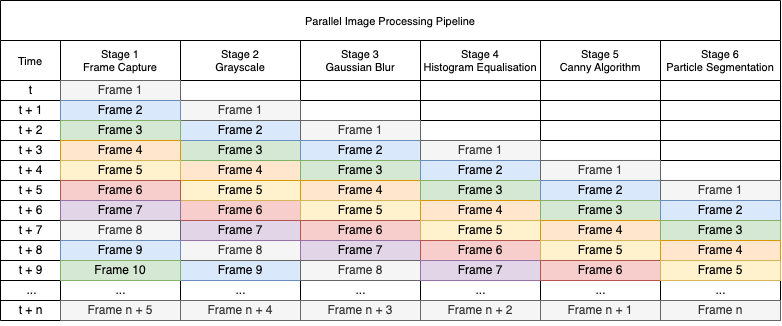
\includegraphics[width=1\textwidth]{assets/image_multiprocessing_pipeline.png}
    \caption{Design for parallel processing in the image processing pipeline for the system.}
    \label{fig:multiprocessing_pipeline}
\end{figure}

In addition to parallel multiprocessing, the system must implement a real-time kernel with the PREEMPT-RT patch. Shepherd's use of the fully-fledged Raspberry Pi OS, which includes a desktop environment and a full software suite, may have been the reason which led to its jitter, primarily due to the OS scheduler preemption type which prioritises a smoother graphical user interface over system latencies, and also due to the vast number of bundled software which could have been consuming CPU time. To ensure minimal OS and software overhead, I will be using the 64-bit Raspberry Pi OS Lite, which does not come with a desktop environment or any non-dependency software. Applying the PREEMPT-RT patch to the OS will reduce stage durations due to the reduction in system latency, and additionally, will also reduce latency randomness, ultimately improving system real-time and predictability. The final key factor is the ability to control the system frame rate, essentially by adding a delay to ensure processing at the established rate. For this design, the implementation must track the duration of each stage accurately to compute the necessary delay duration.
